\documentclass{article}

\usepackage{amsmath}
\usepackage[margin=3cm]{geometry}
\usepackage{graphicx}
\usepackage{hyperref}
\usepackage{listings}
\usepackage{minted}
\usepackage[nodayofweek]{datetime}

\title{
    \textbf{Programming Club}\\
    Ray Tracing \\
}
\author{Hugh Leather}
\date{\today}

\begin{document}
    \maketitle

\setlength{\parskip}{1em}
\setlength{\parindent}{0em}

    \section{Problem description}
        Build a simple ray tracer in any language you like.
            
    \section{Introduction}
        Reverse ray tracing 
        
        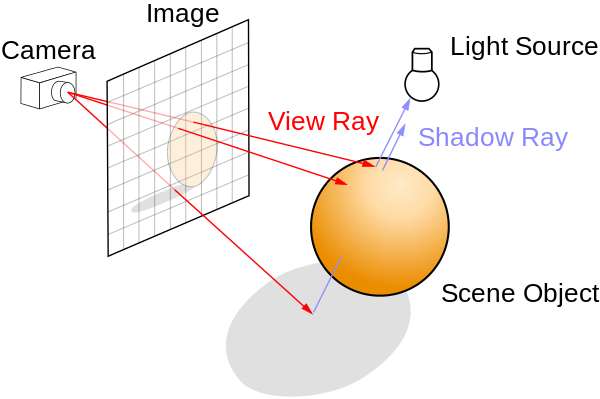
\includegraphics[width=0.3\textwidth]{tracing}
        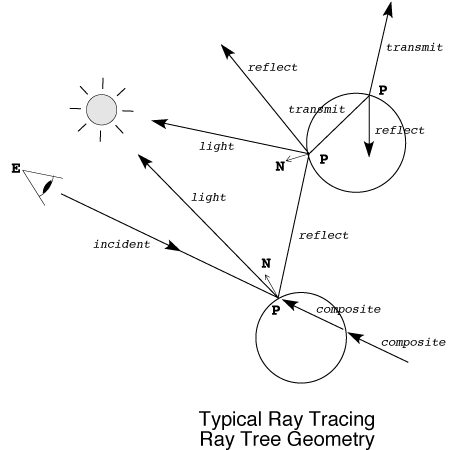
\includegraphics[width=0.3\textwidth]{tree}
    
    \section{Some maths}
        \subsection{Dot product}
            \begin{align*}
                \mathbf{a} \cdot \mathbf{b} &= (a_x,a_y,a_z) \cdot (b_x,b_y,b_z)\\
                                            &= a_xb_x + a_yb_y + a_zb_z\\
                                            &= \lVert\mathbf{a}\rVert \lVert\mathbf{b}\rVert cos \theta
            \end{align*}
        \subsection{Length of vector}
            $\lVert\mathbf{x}\rVert = \sqrt{\mathbf{x} \cdot \mathbf{x}}$
        \subsection{Reflection}
            Incident vector, $\mathbf{x}$, surface normal, $\mathbf{n}$.
            
            Reflected vector is $\mathbf{r} = \mathbf{x} - 2\mathbf{n}(\mathbf{x}\cdot\mathbf{n})$
        \subsection{Refraction}
            Incident vector, $\mathbf{x}$, surface normal, $\mathbf{n}$. 
            Refractive index of original medium, $\gamma_1$, of new medium, $\gamma_2$.
            
            Let
            \begin{align*}
                \gamma &= \gamma_1 / \gamma_2\\
                c_1 &= \mathbf{x}\cdot\mathbf{n}\\
                c_2 &= \sqrt{1 - \gamma^2 * (1 - c_1^2)}
            \end{align*}
            
            Refracted vector is $\mathbf{r} = (\gamma * \mathbf{x}) + (\gamma * c_1 - c_2) * \mathbf{n}$
        \subsection{Intersection of ray and sphere}
            Sphere is centred at $\mathbf{p_c}$, radius $r$.
            Ray origin at $\mathbf{p_0}$, direction $\mathbf{d}$.
            
            Let:
            \begin{align*}
                a &= \mathbf{d} \cdot \mathbf{d}\\
                b &= 2 \mathbf{d} \cdot (\mathbf{p_0} - \mathbf{p_c})\\
                c &= (\mathbf{p_0} - \mathbf{p_c}) \cdot (\mathbf{p_0} - \mathbf{p_c}) - r^2
            \end{align*}
            
            Intersection at $t = \cfrac{-b \pm \sqrt{b^2 - 4 a c}}{2 a}$
        \subsection{Intersection of ray and plane}
            Plane has normal $\mathbf{n}$ and $c$ (gives implict eqn $\mathbf{n}\cdot\mathbf{p}+c=0$)
            
            Ray origin at $\mathbf{p_0}$, direction $\mathbf{d}$.
            
            Intersection at $t = -\cfrac{c + \mathbf{n} \cdot \mathbf{p_0}}{\mathbf{n} \cdot \mathbf{d}}$
            
        \subsection{Lighting and shading}
            Energy from point source is inversely proportional to distance squared.  Tends to be very dark, consider lower exponent than 2.
            
            Energy per unit area proportional to $cos\theta$, where $\theta$ is angle between surface normal and light source.
            
            Note, this simple model will be a bit rubbish.  Consider adding ambient light
            
            Shadows if object intersects ray from object to light.
            
            Reflection and refraction can spawn a new ray each - have a depth threshold.
            
            Note simple checkerboard patterns are easy, based on where the point is in space.
                    
    \section{Output}
        The simplest picture format you might use is PPM.  You can, however use any way to show the ray traced image you like.
        
        The PPM format is:
        \begin{itemize}
            \item A ``magic number'' for identifying the file type. A ppm image's magic number is the two characters ``P6''.
            \item Whitespace (blanks, TABs, CRs, LFs).
            \item A width, formatted as ASCII characters in decimal.
            \item Whitespace.
            \item A height, again in ASCII decimal.
            \item Whitespace.
            \item The maximum colour value (Maxval), again in ASCII decimal. Must be less than 65536 and more than zero.
            \item A single whitespace character (usually a newline).
            \item A raster of Height rows, in order from top to bottom. Each row consists of Width pixels, in order from left to right.
            Each pixel is a triplet of red, green, and blue samples, in that order. Each sample is represented in pure binary by either 1
            or 2 bytes. If the Maxval is less than 256, it is 1 byte. Otherwise, it is 2 bytes. The most significant byte is first.
            \item A row of an image is horizontal. A column is vertical. The pixels in the image are square and contiguous.
        \end{itemize}
        
   

\end{document}
